
\chapter{Using the MGX application}
\label{using}

\section{Basic concepts}

\subsection{Metadata}

In addition to the sequence data, MGX requires a user to provide additional information
about a dataset, e.g. further details about the investigated habitat as well as sampling
and sequencing procedures. Metadata in the MGX platform is organized in a hierarchical
manner describing

\begin{itemize}
  \item the geographical location of a habitat,
  \item the sample taken from a habitat,
  \item the DNA extraction procedure,
  \item sequencing technology and protocol.
\end{itemize}

\subsection{Read-based analysis: Attributes and attribute types}

\section{Obtaining a MGX project}

Currently, there is no way to automatically create new MGX projects. If you would like to
analyse your data using MGX, send a mail to the MGX team, which can be contacted at 
\href{mailto:mgx@CeBiTec.Uni-Bielefeld.DE}{mgx@CeBiTec.Uni-Bielefeld.DE}. MGX projects
and users are managed by the General Project Management System (GPMS) developed at CeBiTec,
which provides Single Sign-On (SSO) for all applications provided by CeBiTec's Computational
Genomics group.

To apply for a new project, include information about

\begin{itemize}
  \item suggested \textit{project name}, e.g. MGX\_AcidMine
  \item a short \textit{one-line description} of your project (''Acid Mine Drainage metagenome'')
  \item a \textit{contact address} of a single person responsible for the project (PI or group leader)
  \item a \textit{list of all users} that should be granted project access, including
    \begin{itemize}
      \item Full name and email address for users not yet registered in the GPMS system, GPMS username otherwise
      \item desired access level
    \end{itemize}
\end{itemize}

MGX offers different access levels (roles), which are assigned individually for each
project: \\

\begin{itemize}
  \item{\textbf{Admins} are equal to Users (see below), but can grant access to additional users.}
  \item \textbf{Users} have full access to a MGX project and are able to define new or modify
present datasets, import new sequences and execute analysis jobs. They are also able to
delete all data associated with a project.
  \item \textbf{Guests} are provided read-only access to a project, i.e. they are able to access
all information already present, view analysis results and export data; however, they are
unable to perform new analysis or delete data from the project.
\end{itemize}

As new users can always be added to an existing MGX project, all registered users are required
to carefully protect their login credentials and not to share them with any third party.

\section{Connecting to a MGX server}

\begin{figure}[ht]
\centering
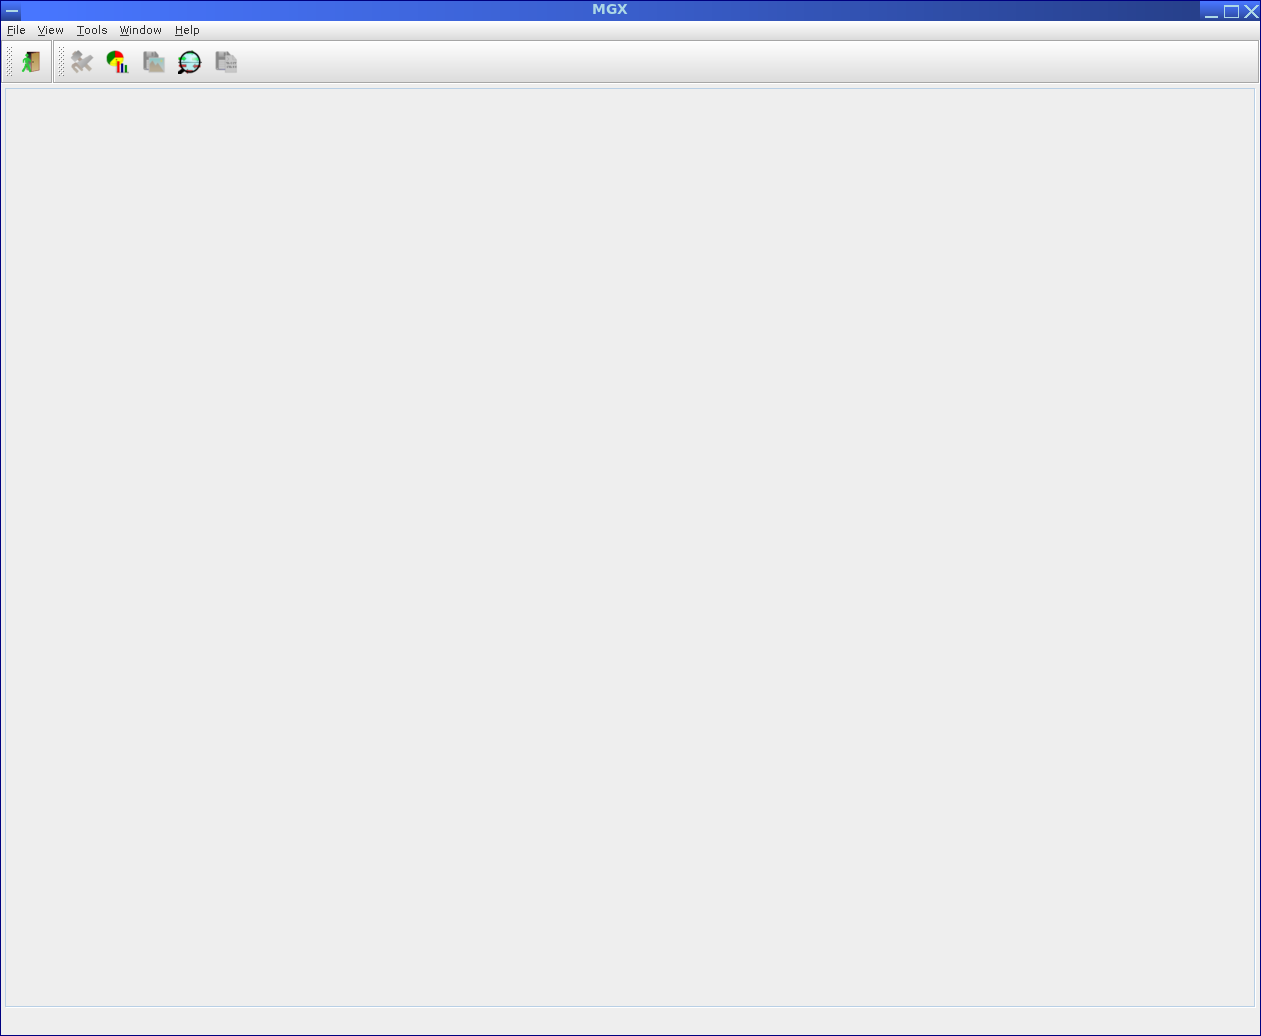
\includegraphics[width=.8\textwidth]{img/mgx/startup}
\caption[MGX client]{Screenshot of the client application right after startup.}
\label{startup}
\end{figure}

After installation, the MGX application is already preconfigured to connect to the 
MGX server instance hosted at CeBiTec, Bielefeld University. In case a different MGX server
should be used, the default server can be changed choosing Tools \textrightarrow Options from the menu
and navigating to the MGX server tab (\ref{config-site}). While the site name can be freely
chosen by the user, the server URL has to be entered as provided by the site administrators.

\begin{figure}[ht]
\centering
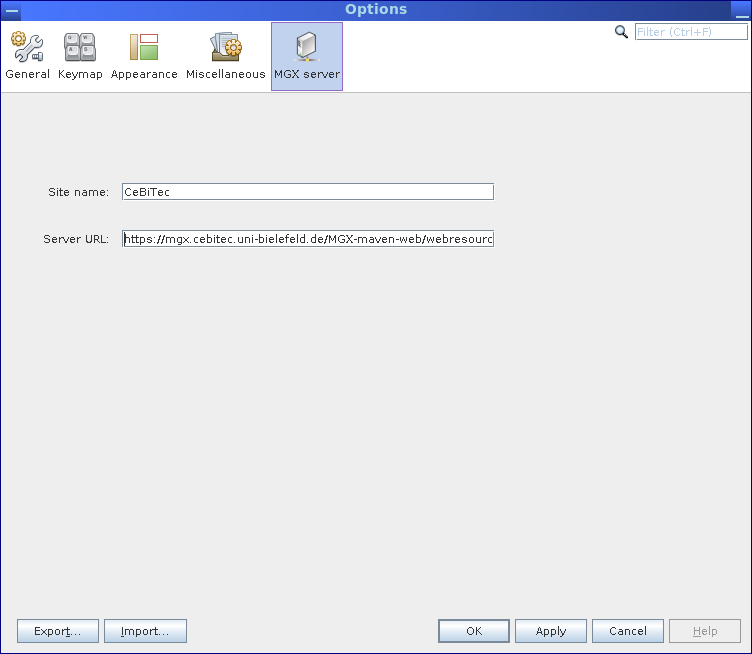
\includegraphics[width=.8\textwidth]{img/mgx/config-site}
\caption[Server configuration]{A different default server instance can optionally be configured in the MGX 
server tab, which is available from the Tools \textrightarrow Options menu.}
\label{config-site}
\end{figure}


\begin{figure}[H]
\centering
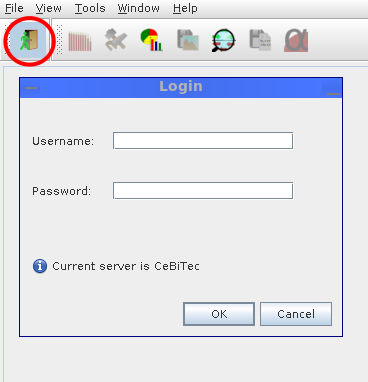
\includegraphics[width=.6\textwidth]{img/mgx/login}
\caption[Login screen]{The first button in the menu toolbar will bring up the login dialog, allowing to connect to the configured server; the login screen also reflects the name of the current server.}
\label{login-screen}
\end{figure}

All communication between the MGX user interface and the MGX server is encrypted using
the standardized SSL (Secure Sockets Layer) protocol, ensuring confidentiality of 
unpublished data and protecting the integrity of login credentials.
%\section{Browsing and exploring MGX projects}
After successfully logging in, a new window is automatically opened. The MGX Explorer window
lists all available projects a user is allowed to access, including both public as well as
private projects. Projects are easily opened or closed by simply expanding the corresponding
nodes in the Project Explorer window (\ref{projects}).\\

\begin{figure}[H]
\centering
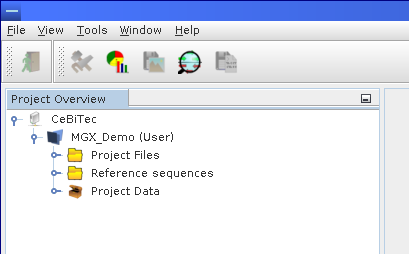
\includegraphics[width=.8\textwidth]{img/mgx/projects}
\caption[Project Explorer]{After successful login, the Project Explorer component will automatically open,
showing a list of MGX projects available to the current user. Shown is just one project, MGX\_Demo, with
access level indicated behind the project name.}
\label{projects}
\end{figure}

\begin{figure}[H]
\centering
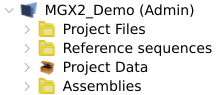
\includegraphics[width=.4\textwidth]{img/mgx/projstructure}
\caption[Project structure]{Divided into three different parts, a MGX projects offers
(from top to bottom) dedicated storage for files to be used by analysis pipelines, 
managed reference sequences (including annotation data, if available) and general
project data containing metadata as well as sequence datasets.}
\label{structure}
\end{figure}

Each project contains metagenome datasets as well as structured storage (\ref{structure}), where user-provided
databases can be uploaded to be used in custom analysis pipelines (Chapter \ref{custom}).

\section{Creating a new habitat}

New habitats are defined choosing ''Add habitat'' (\ref{addhabitat}) from the context menu of the ''Project Data''
node. This will bring up a wizard allowing to select the corresponding geographical location as well as
specifying a habitats name and biome type (\ref{habwiz}). In a second step, an optional description for this
habitat may be entered, as well.

\begin{figure}[H]
\centering
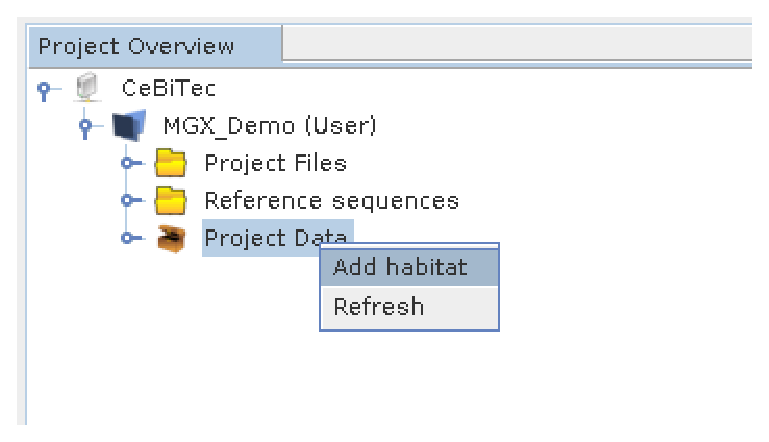
\includegraphics[width=.4\textwidth]{img/mgx/addhabitat}
\caption[Habitat creation]{A new habitat can be added selecting the appropriate entry from the context
menu of the ''Project Data'' node.}
\label{addhabitat}
\end{figure}

\begin{figure}[H]
\centering
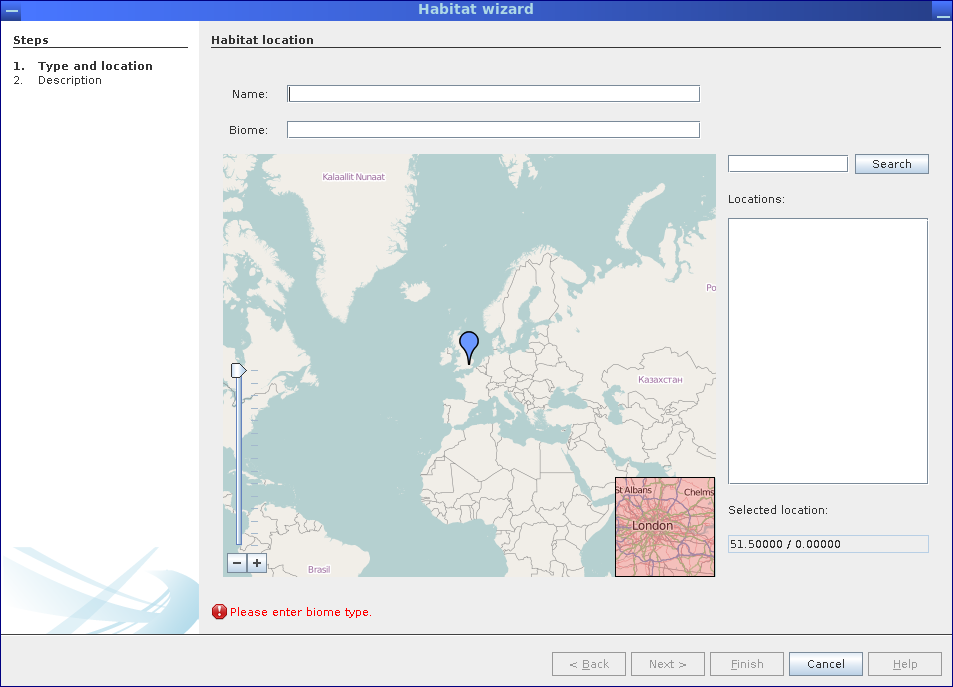
\includegraphics[width=.8\textwidth]{img/mgx/habwizard}
\caption[Habitat wizard]{The habitat wizard allows to define new habitats specifying their location, name and
biome type.}
\label{habwiz}
\end{figure}

\section{Creating new samples and DNA extracts}

Samples and DNA extracts are created in the same way as habitats, except that samples are defined for
habitats and DNA extracts are defined based on samples. Thus, the corresponding wizards are available
from the context menu of the ''Habitat'' and ''Sample'' nodes, respectively.

\begin{figure}[H]
\centering
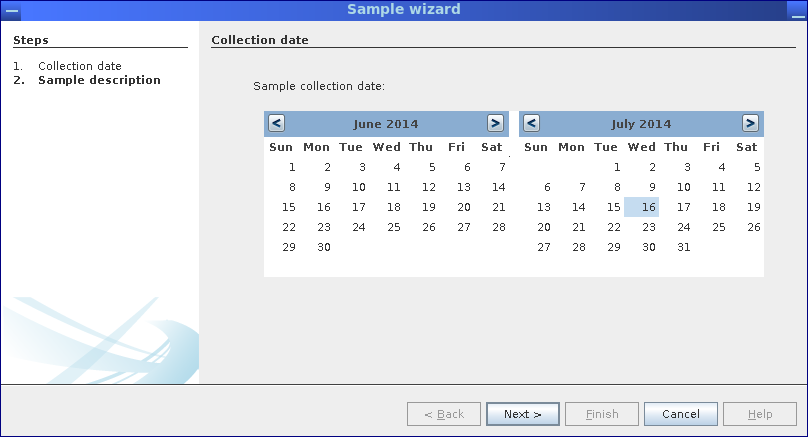
\includegraphics[width=.8\textwidth]{img/mgx/samplewiz1}
\caption[Sample wizard]{In the first step of the sample wizard, the sampling date is selected.}
\label{samplewiz1}
\end{figure}

\begin{figure}[H]
\centering
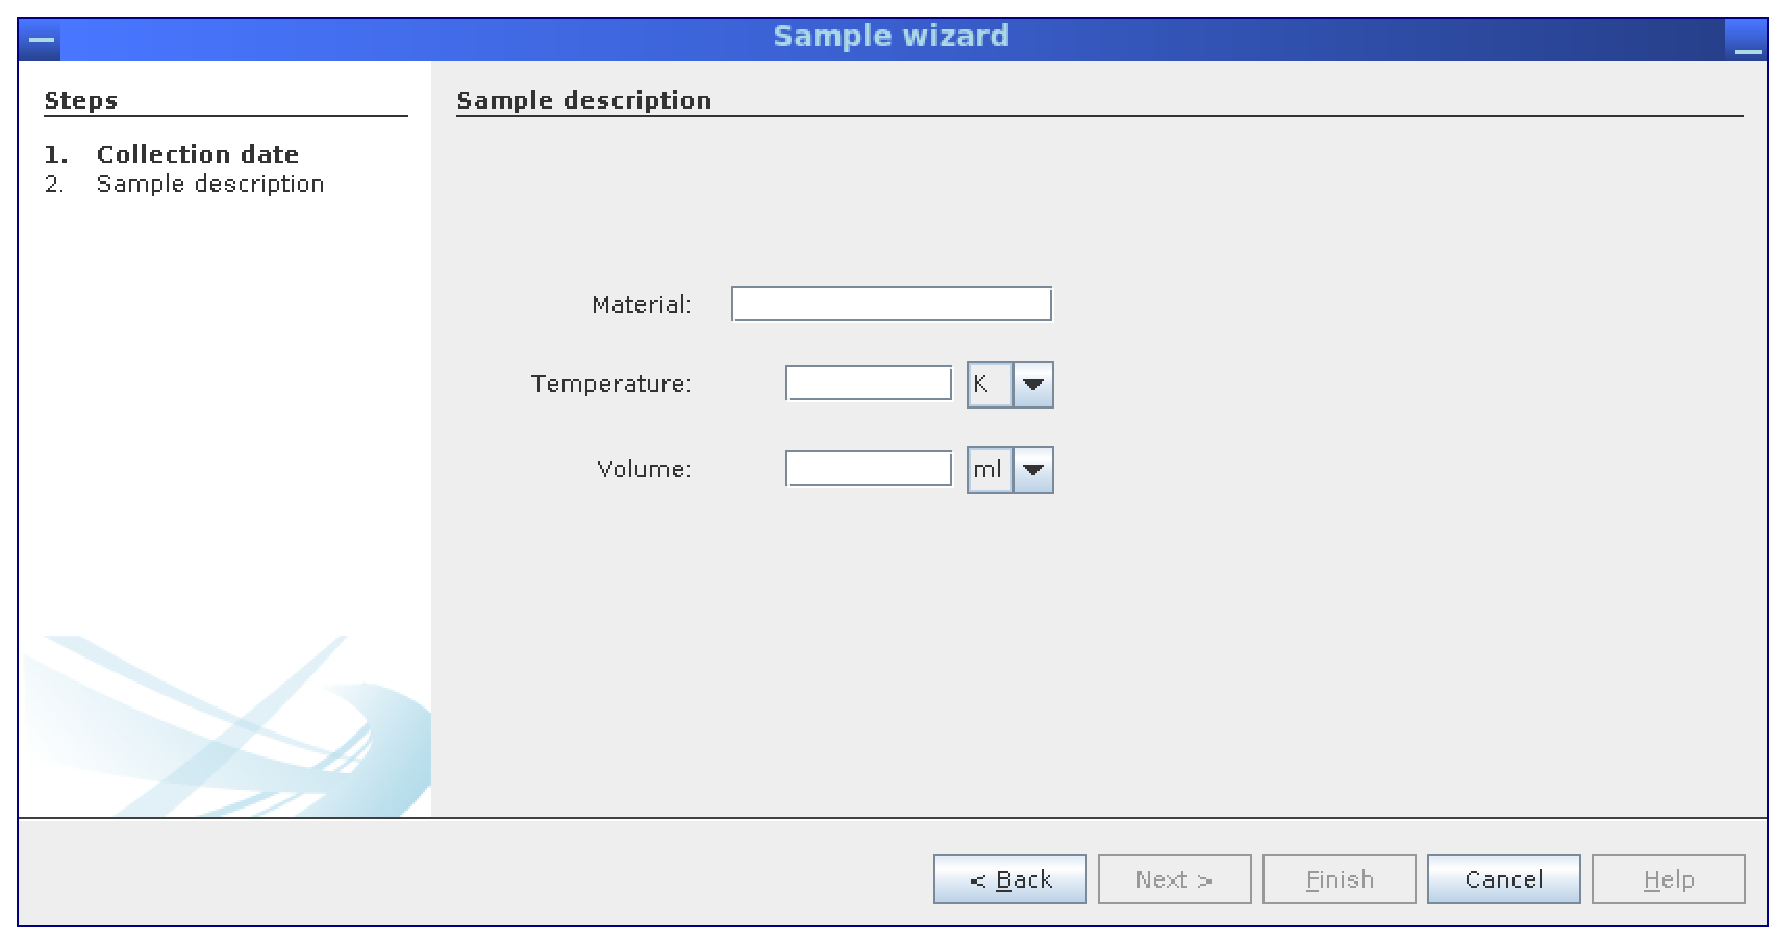
\includegraphics[width=.8\textwidth]{img/mgx/samplewiz2}
\caption[Sample wizard]{In the second step, the sampled material as well as temperature and sampled volume/weight
need to be entered.}
\label{samplewiz2}
\end{figure}

\begin{figure}[H]
\centering
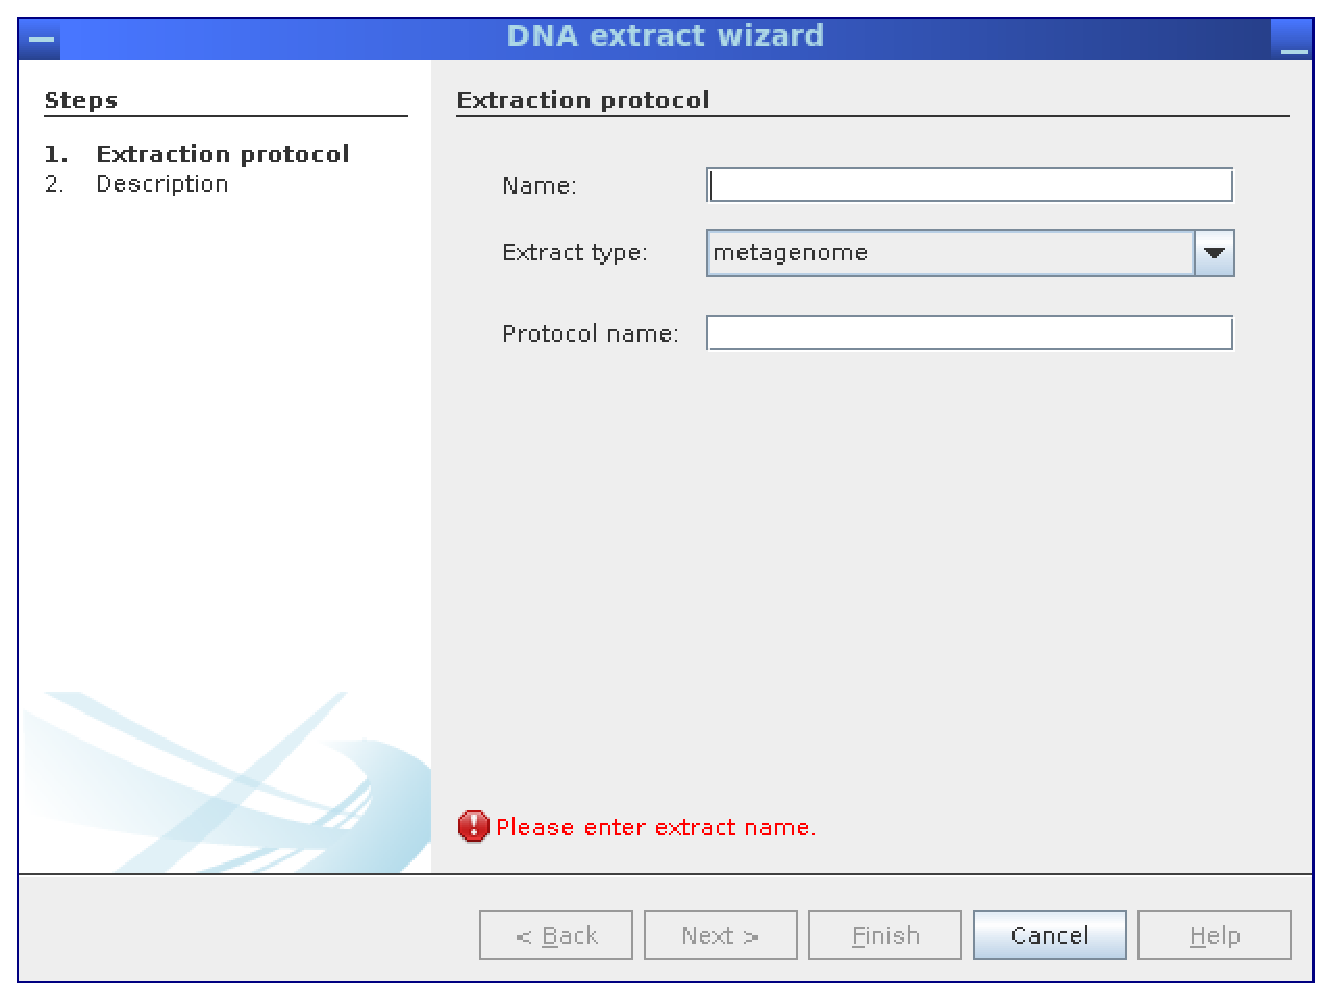
\includegraphics[width=.8\textwidth]{img/mgx/extractwiz1}
\caption[DNA extract wizard]{The DNA extract wizard allows to specify the type of DNA extract (metagenome, 
metatranscriptome, amplicon) and protocols used to extract the DNA.}
\label{extractwiz1}
\end{figure}

\begin{figure}[H]
\centering
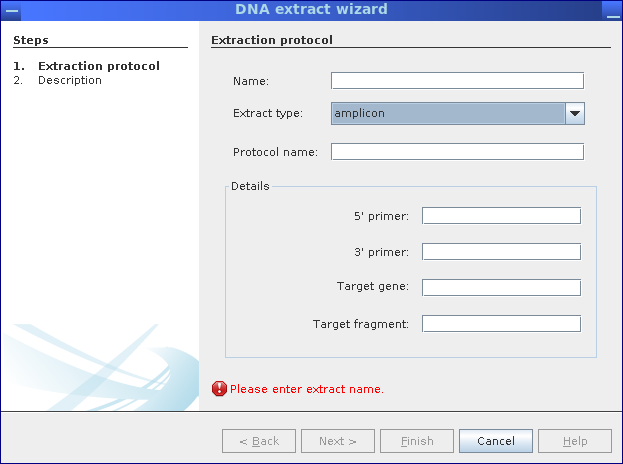
\includegraphics[width=.8\textwidth]{img/mgx/extractwiz2}
\caption[DNA extract wizard]{Depending on DNA extract type, additional data can be entered; for amplicons, primer
names and the corresponding target gene (fragment) can be entered, for metatransriptomes, the type of RNA depletion
methods can be selected.}
\label{extractwiz2}
\end{figure}

\section{Importing sequence data}

\begin{figure}[H]
\centering
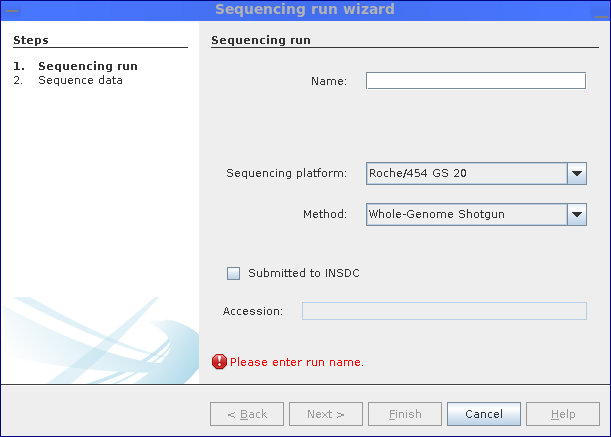
\includegraphics[width=.8\textwidth]{img/mgx/runwiz1}
\caption[Sequence import]{Before sequence data can be uploaded, the employed sequencing platform and technology have 
to be specified; for data already submitted to or obtained from public repositories, the corresponding accession
number can be added, as well.}
\label{dnawiz1}
\end{figure}

\begin{figure}[H]
\centering
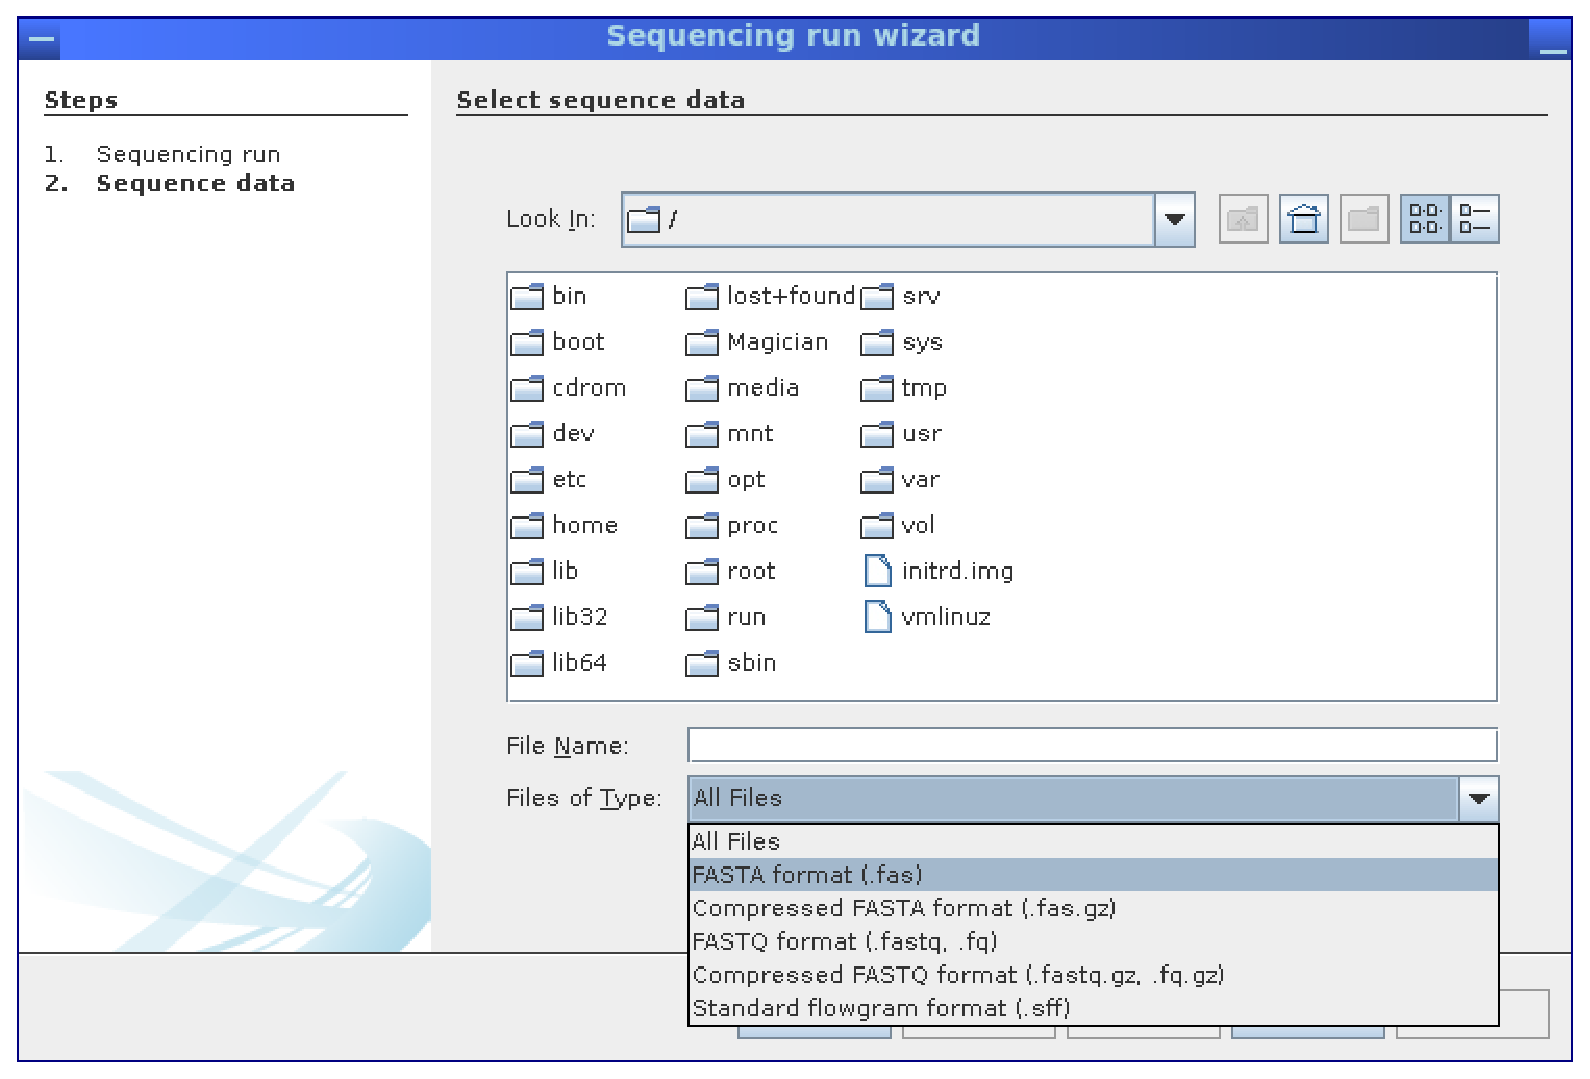
\includegraphics[width=.8\textwidth]{img/mgx/runwiz2}
\caption[Sequence import]{Finally, the file containing the sequence data is selected; MGX supports all commonly used
file formats such as FASTA, FASTQ, or SFF.}
\label{dnawiz2}
\end{figure}

\section{Quality control}

After sequence import, Quality control reports generated within MGX should be inspected. 
MGX currently offers three types of QC reports: Distribution of GC content, sequence length
and nucleotide distribution within the DNA sequences. Those can be used to evaluate overall
sequence data quality and check for possible signs of contamination.

TODO: icon for QC

Data shown relates to the artificial \textbf{simHC} metagenome dataset created by the
FAMeS\cite{SIMMETA} project. The acutal sequence data can be obtained from \url{http://fames.jgi-psf.org/Retrieve_data.html}.

\begin{figure}[H]
\centering
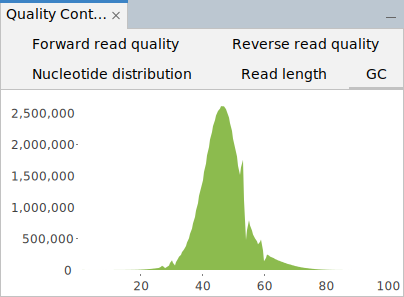
\includegraphics[width=.8\textwidth]{img/mgx/QCgc}
\caption[Quality control]{GC distribution of the simHC dataset.}
\label{qc1}
\end{figure}

\begin{figure}[H]
\centering
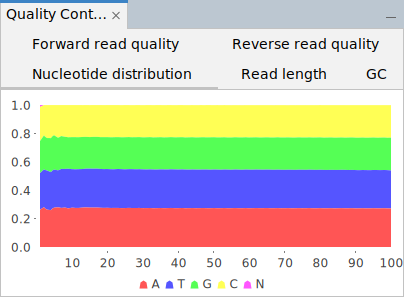
\includegraphics[width=.8\textwidth]{img/mgx/QCnuc}
\caption[Quality control]{Nucleotide distribution of the simHC dataset. A high fraction of uncalled bases
is apparent from the chart.}
\label{qc2}
\end{figure}

\begin{figure}[H]
\centering
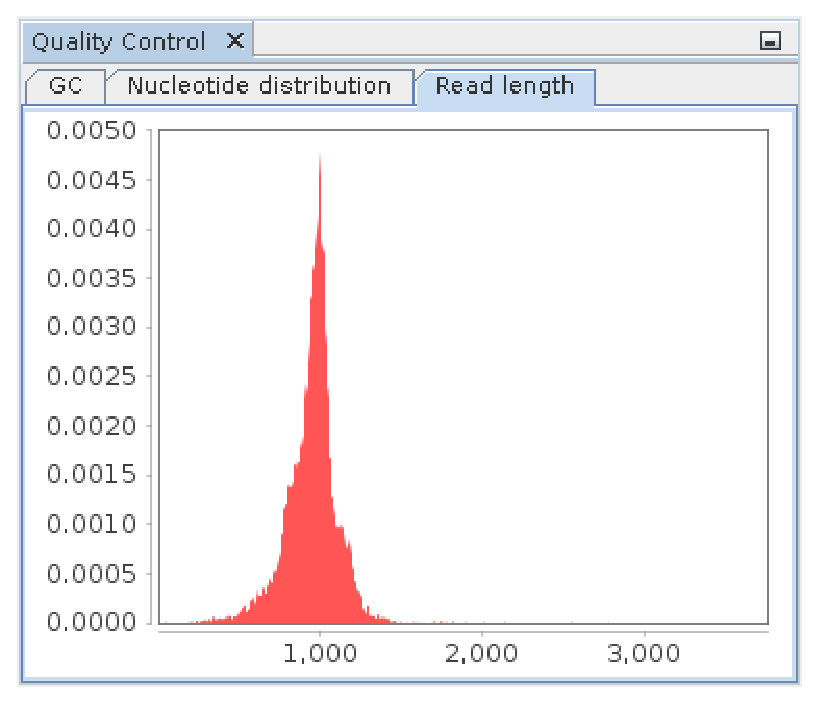
\includegraphics[width=.8\textwidth]{img/mgx/QCreadlen}
\caption[Quality control]{Read length distribution of the simHC dataset. }
\label{qc3}
\end{figure}

\subsection{Examples}

\begin{figure}
        \centering
        \begin{subfigure}[b]{0.3\textwidth}
                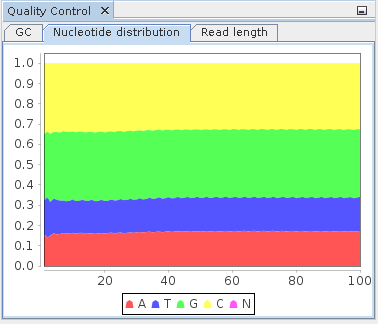
\includegraphics[width=\textwidth]{img/mgx/highGCnucl}
                \caption{High-GC (65\%) data}
        \end{subfigure}%
        \begin{subfigure}[b]{0.3\textwidth}
                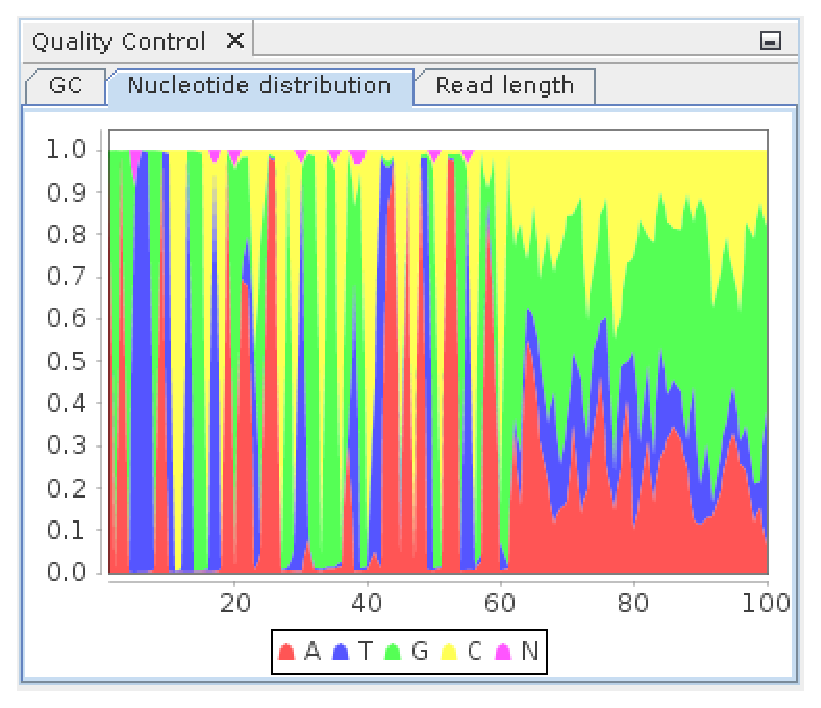
\includegraphics[width=\textwidth]{img/mgx/ampliconNucl}
                \caption{Amplicon data}
        \end{subfigure}
        \begin{subfigure}[b]{0.3\textwidth}
                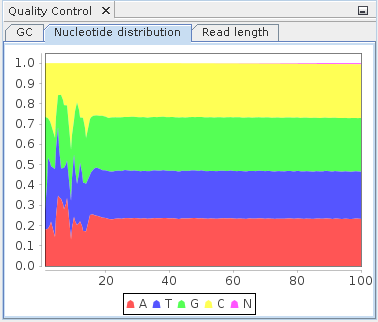
\includegraphics[width=\textwidth]{img/mgx/adapterNucl}
                \caption{Adapter residue}
        \end{subfigure}
        \caption{Nucleotide distribution examples}
\end{figure}



\section{Defining and executing analysis jobs}

\begin{figure}[H]
\centering
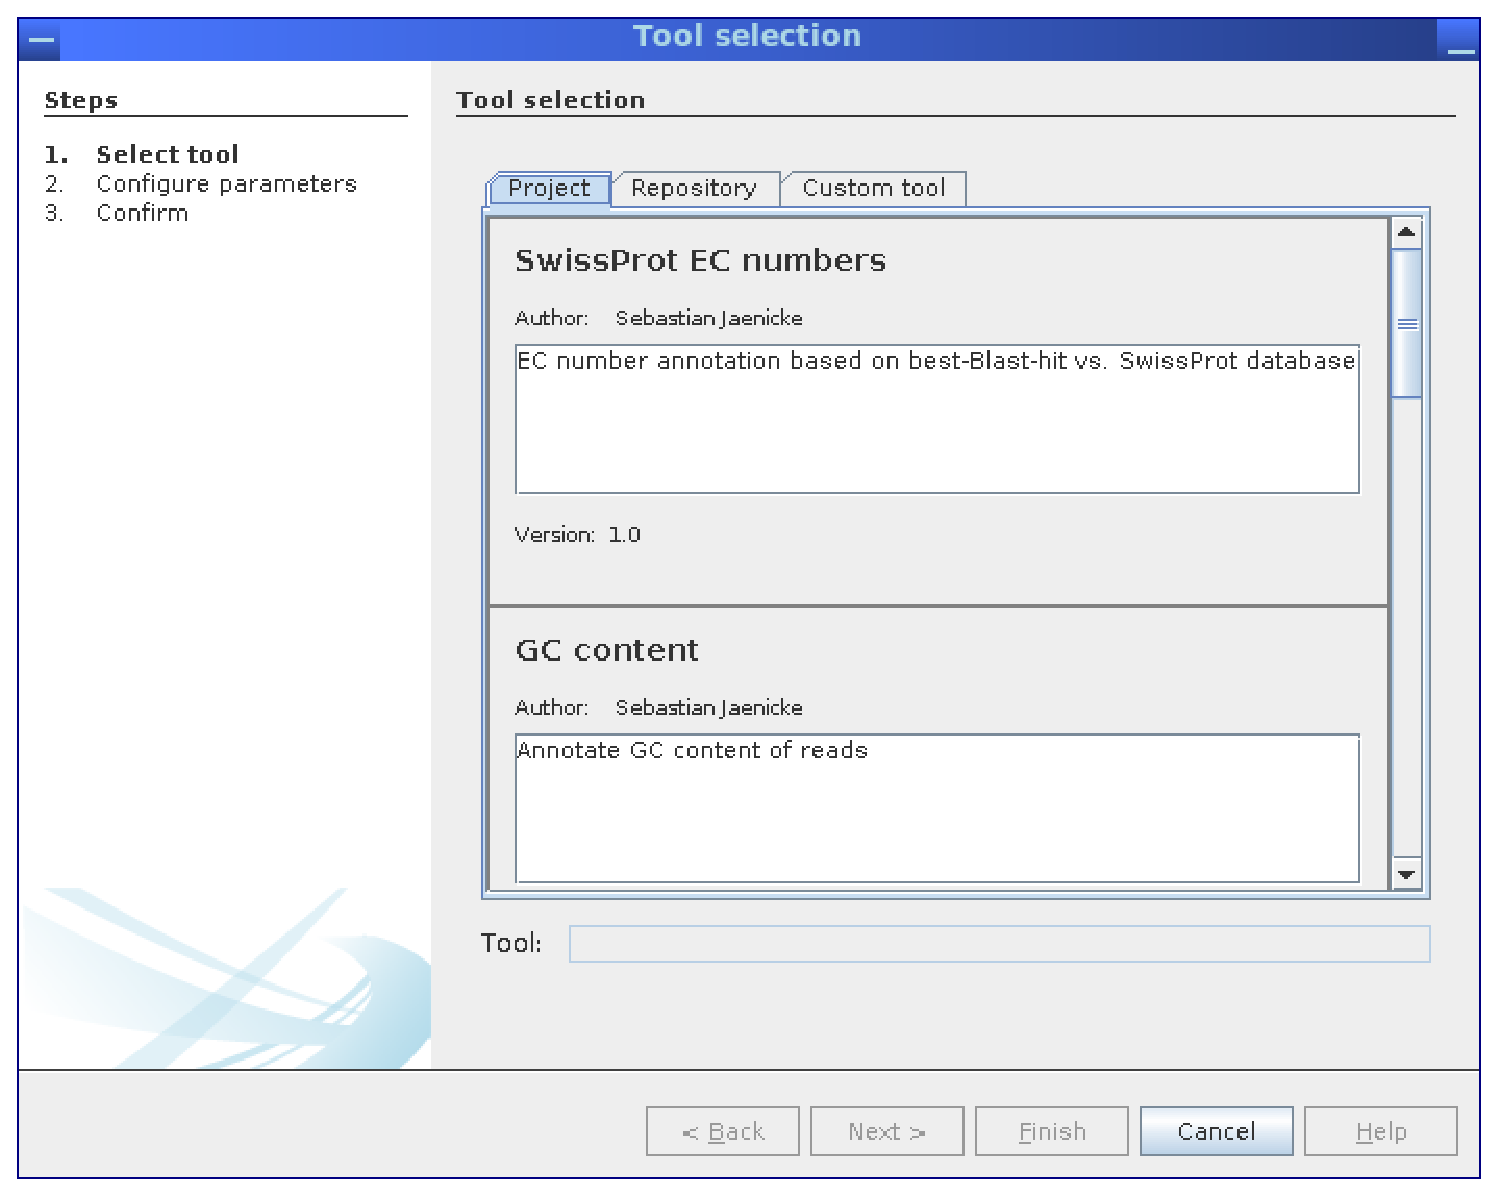
\includegraphics[width=.8\textwidth]{img/mgx/analysiswiz1}
\caption[Analysis selection]{TODO}
\label{anawiz1}
\end{figure}

All analysis pipelines can be started from the context menu of the metagenome dataset to be analyzed. First,
the used can choose the desired pipeline from the project itself, from the pipeline repository hosted on the
MGX server, or upload an own pipeline implementation (\ref{anawiz1}). Subsequently, analysis parameters
can be reviewed and adapted (\ref{anawiz2}) before submitting an analysis.

\begin{figure}[H]
\centering
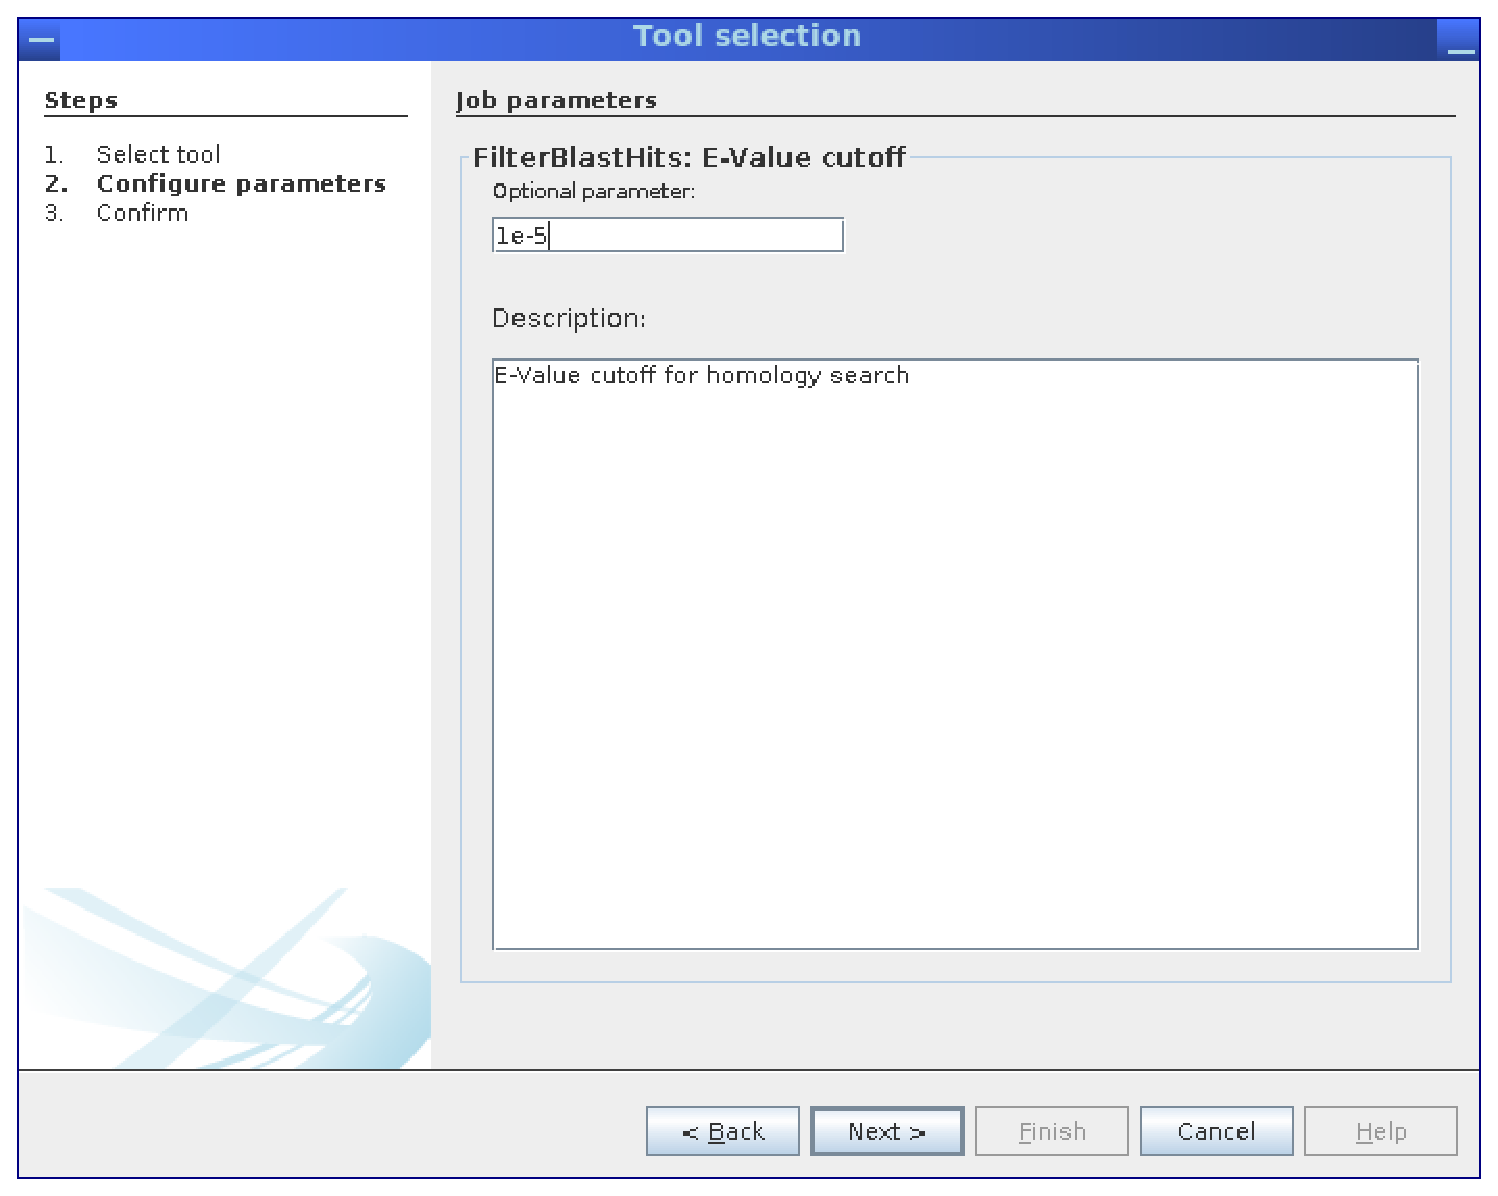
\includegraphics[width=.8\textwidth]{img/mgx/analysiswiz2}
\caption[Analysis parameters]{The wizard allows to inspect and adapt parameters for the selected pipeline. The actual
number of steps depends on the number of parameters available for customization.}
\label{anawiz2}
\end{figure}

\begin{figure}[H]
\centering
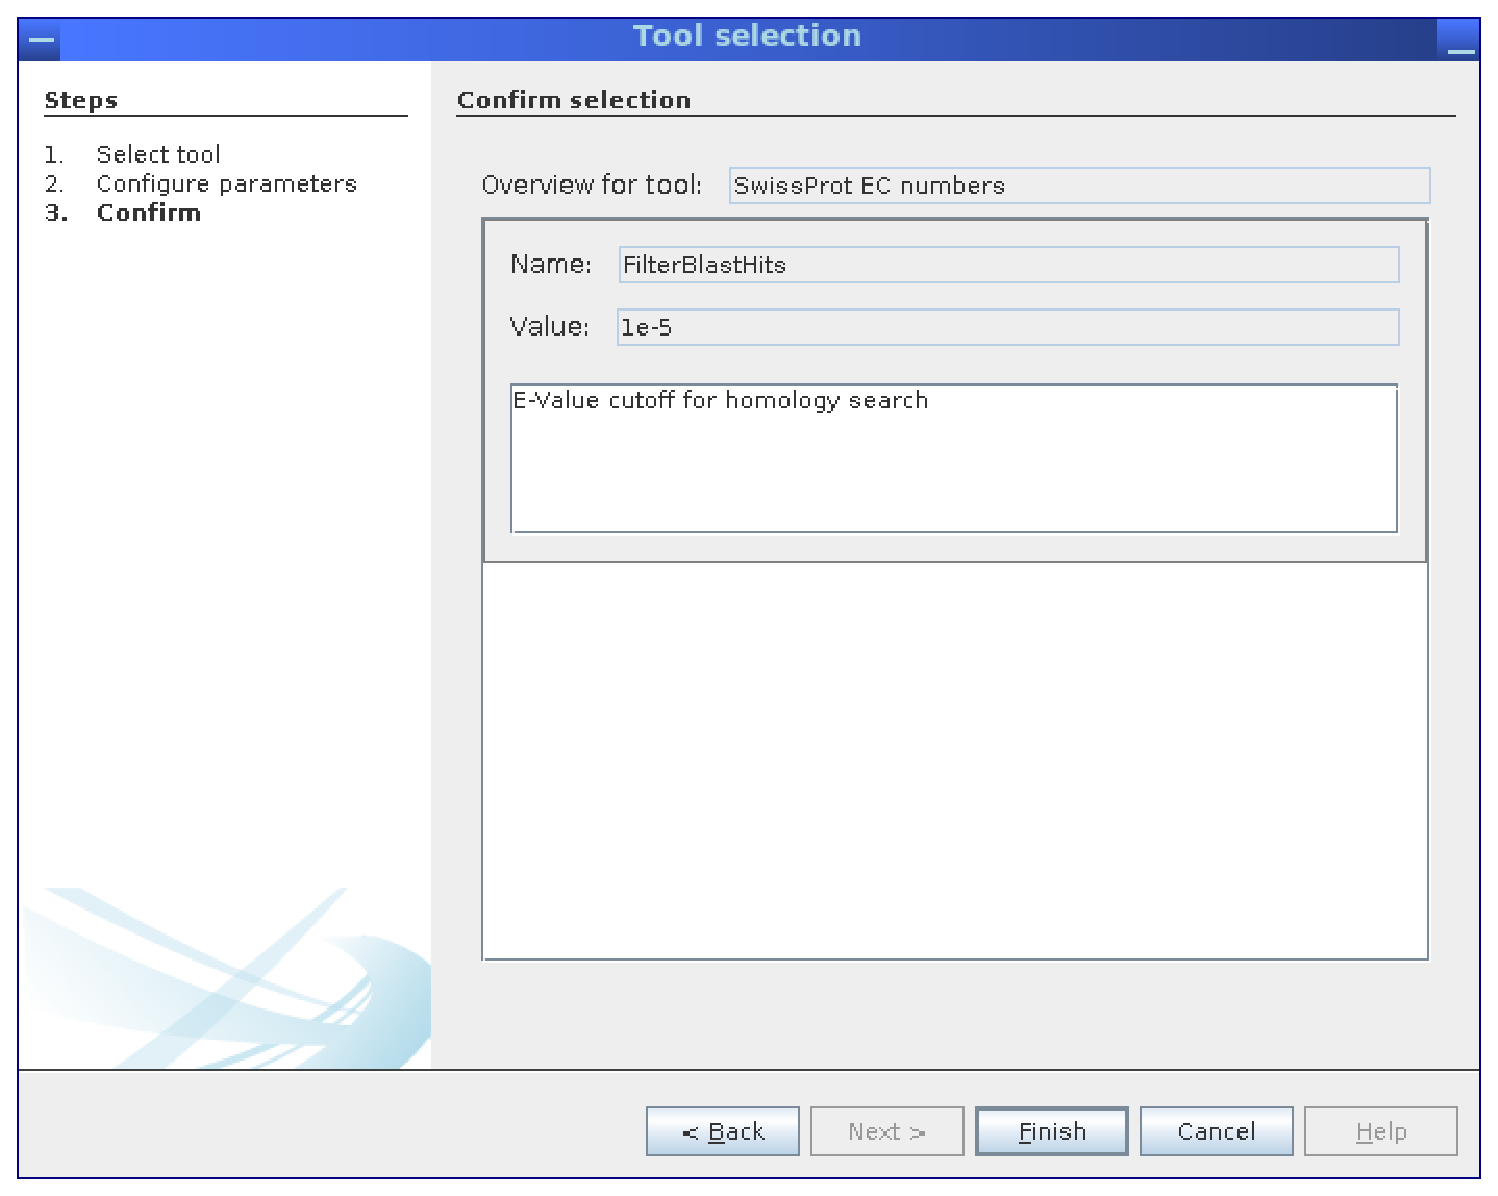
\includegraphics[width=.8\textwidth]{img/mgx/analysiswiz3}
\caption[Parameter overview]{Before executing an analysis pipeline, a final overview of all parameters is shown. Once
confirmed, the pipeline is submitted and scheduled for execution on the MGX server. Here, the selected pipeline has
only one single parameter.}
\label{anawiz3}
\end{figure}

\subsection{Monitoring job progress}
\section{Visualization of results}
\subsection{Choosing data sets}
\subsection{Choosing a visualisation type}
\subsection{Exporting sequences}
\section{Search}


